\documentclass[12pt,a4paper]{article}
\usepackage[utf8]{inputenc}
\usepackage{amsmath}
\usepackage{amsfonts}
\usepackage{amssymb}
\usepackage{graphicx}

\usepackage{float}
\usepackage{hyperref}

\title{Homework 2 - Model Predictive Control}
\author{Erivelton Gualter dos Santos}
\date{}

\begin{document}
\maketitle 

\section{Mini-Project - Elevator}

In order to verify that the discrete states have the same physical meaning as their continuous counterparts, a simulation was done in order to compare both states after discretization for a sinusoidal control input. 

\begin{figure}[H]
	\centering
    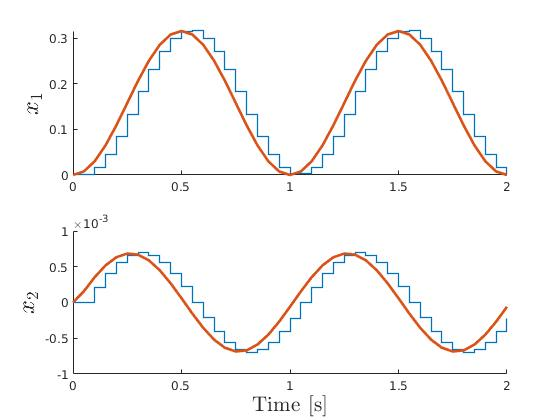
\includegraphics[width=0.9\textwidth]{compare.jpg}
\end{figure}

The code to verify the discretization can be found here: \url{https://github.com/EriveltonGualter/ESC-794-Model-Predictive-Control/tree/master/HW2}.

\subsection{Tuning Control System}

In order to help the task to control the system, it was developed a interface, which is despited in the following figure, to accelerate and simplify the process to tune the parameters. 

\begin{figure}[H]
	\centering
    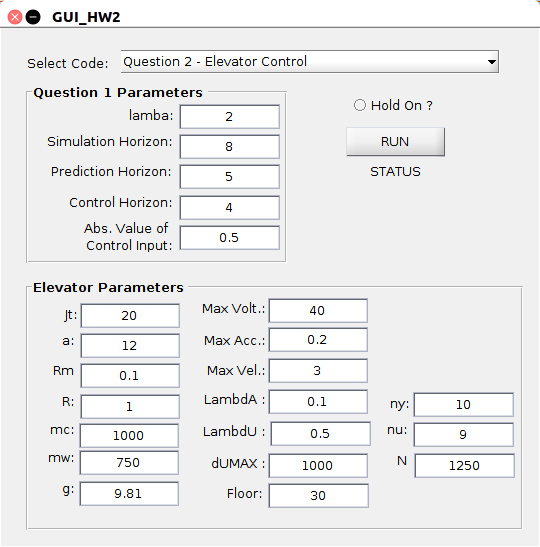
\includegraphics[width=0.9\textwidth]{GUI.png}
    \caption{Interface for Homework 2}
\end{figure}

After some tests varying the parameters of the MPC controller ($\lambda$ and $\lambda_u$), it was clear that for the current specifications of the problem we ca not achieve it. In order to reach all the requirements, it is necessary to alter some of the constraints for example. 

Next figure contains the results of the controller. 

\begin{figure}[H]
	\centering
    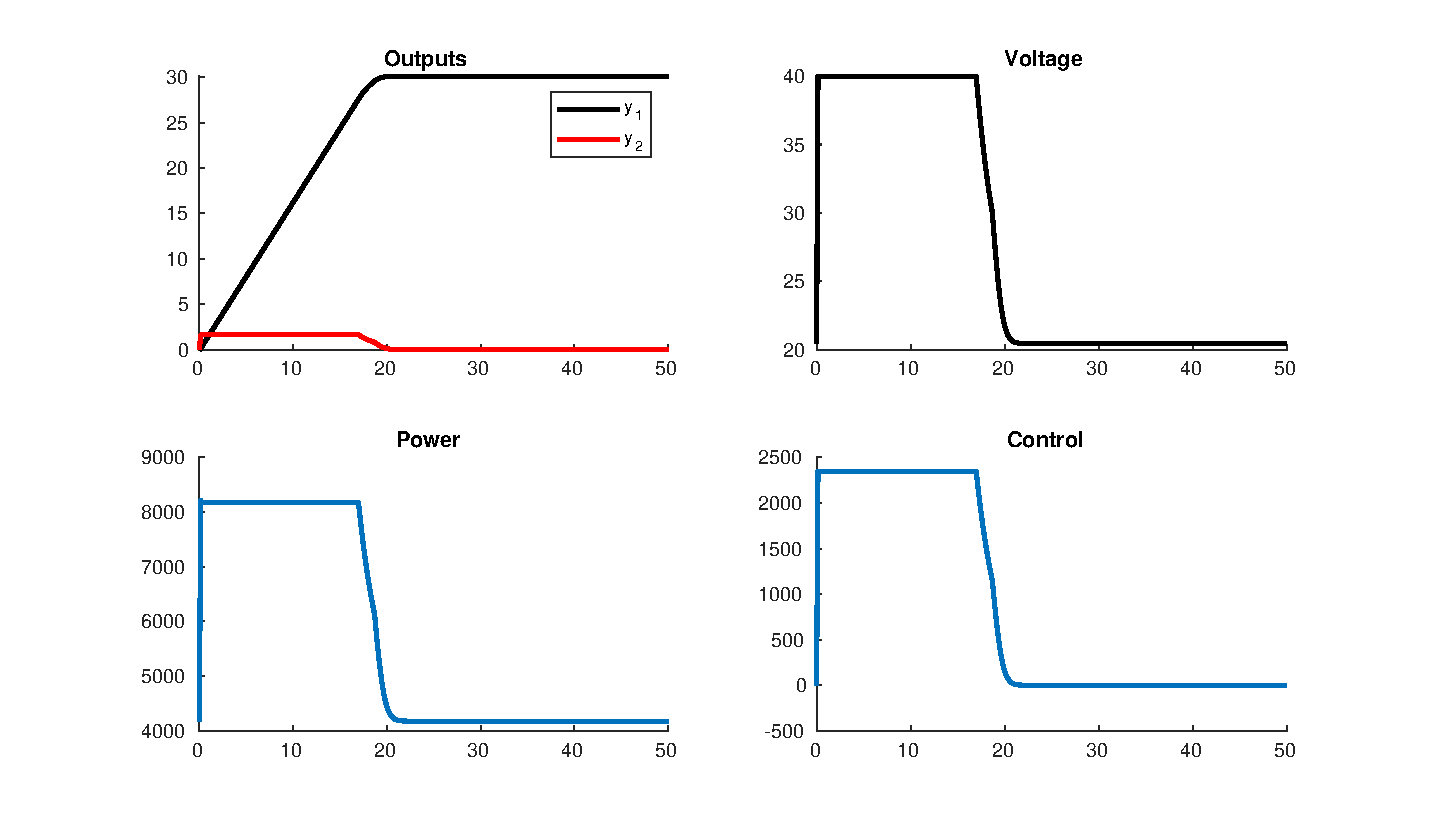
\includegraphics[width=\textwidth]{elevator.eps}
    \caption{Results}
\end{figure}

\textbf{References}
\begin{enumerate}
\item \url{https://www.thyssenkruppelevator.com/Tools/energy-calculator}
\end{enumerate}

\end{document}